
\documentclass[a4paper]{scrreprt}


\usepackage{tabulary } 
\usepackage[german]{babel}
\usepackage[utf8]{inputenc}
\usepackage[T1]{fontenc}
\usepackage{ae}
\usepackage[bookmarks,bookmarksnumbered]{hyperref}
%graphics
\usepackage{graphicx}
\graphicspath{ {images/GUI/c-editor/}
 {images/GUI/Eigenschaften-Liste/}
  {images/GUI/Eigenschaften/}
  {images/GUI/Parameter-editor/}} 

\usepackage[printonlyused]{acronym}
\usepackage{hyperref}
\usepackage{float}

%glossary stuff, must be defined after hyperref
\usepackage[toc]{glossaries}
\makeglossaries

\newglossaryentry{Grundstein}{name=Grundstein,description={Der Demokratie, is klar.}}
\newglossaryentry{CBMC}
{
name={C bounded model checker},
description={Ein Programm, welches C-Programme mit bounded model checking auf Fehler und vom user definierte assertions untersucht}
}



\begin{document}

\title{Pflichtenheft}
\author{Beste Gruppe}
\maketitle
 

\tableofcontents	

\listoffigures

\chapter*{Abkürzungsverzeichnis}
\begin{acronym} %put all your abbreviations here 
\acro{CBMC}{C Bounded Model Checker}
\acro{BMC}{Bounded Model Checking}
\acro{GUI}{Graphical User Interface}
\end{acronym}
 
\chapter{Produktübersicht}
Wahlverfahren bilden den \gls{Grundstein} unserer Demokratie. Dabei werden viele Anforderungen an sie gestellt, welche unsere intuitiven Ideen über Gerechtigkeit formalisieren: Proportionalität, Anonymität, etc. Moderne Wahlverfahren sind oft so komplex, dass sie viele überraschende und teils unerwünschte Eigenschaften haben. Nachweisen deren Abwesenheit ist absolut nicht trivial. So wurde beispielsweise 2008 das Bundestagswahlrecht vom BVerfG für verfassungswidrig erklärt, da es unter anderem Gleichheit der Wirkung verschiedener Stimmen verletzte. Auf der anderen Seite ist es auch sehr schwer, Wahlverfahren auf die Anwesenheit erwünschter Eigenschaften zu untersuchen.

\ac{BMC} Wird normalerweise dazu verwendet zu überprüfen ob ein gegebenes Programm gegebene Eigenschaften erfüllt. Da dieses Problem im Allgemeinen unentscheidbar ist, werden nur endliche Codepfade überprüft. Dadurch wird der Zustandsraum endlich und das Problem entscheidbar. Um dies zu bewerkstelligen, werden potentiell unendliche Codepfade - also Schleifen - bis zu einer vom Benutzer bestimmten Grenze aufgerollt. Danach wird eine SAT-Formel erstellt, die erfüllbar ist genau dann wenn das Programm einen Zustand einnehmen kann welcher die gegebene Eigenschaft nicht erfüllt. Dies ist vollautomatisch und gibt bei Nichterfüllung das Gegenbeispiel zurück.  

In unserem Fall kann \ac{BMC} konkret dazu verwendet werden, ein C-Programm darauf zu untersuchen ob es im Falle gegebener Vorbedingungen gegebene Nachbedingungen erfüllt. Dies wird dazu verwendet, obige Problemstellung zu lösen: so kann ein in C beschriebenes Wahlverfahren wie z.B. die einfache Mehrheitswahl darauf geprüft werden, ob es bestimmte Eigenschaften erfüllt. Allerdings ist es kompliziert, dies direkt zu tun. 

Unser Programm ist im Wesentlichen eine sehr umfangreiche Schnittstelle um mit \ac{CBMC} zu kommunizieren. Es bietet dem Benutzer über eine \ac{GUI} die Möglichkeiten, formale Eigenschaften für Wahlverfahren sowie diese Wahlverfahren selbst anzugeben und zu editieren. Weiterhin liefert es Möglichkeiten die Interaktion mit \ac{CBMC} zu gestalten: Für wie viele Wähler, Plätze etc die Eigenschaft überprüft werden soll. Nach erfolgreicher Überprüfung durch \ac{CBMC} bekommt der Benutzer schließlich eine Antwort des Programms, in der er bei Nichterfüllung der Eigenschaft ein Gegenbeispiel angezeigt bekommt. Wird kein Gegenbeispiel gefunden so wird eine Erfolgsmeldung ausgegeben. All dies wird graphisch über die \ac{GUI} aufbereitet.

Die \ac{GUI} ist nach Funktionalität in vier Teilen angeordnet:
\begin{enumerate}
\item "`Rigtime"': Code-Editor für Wahlverfahren in Programmiersprache C.
\item "Eigenschaften-Liste" Listenansicht aller Eigenschaften, die für dieses Wahlverfahren untersucht werden sollen
\item "`Eigenschaften-Editor"': Editor für Spezifikation formaler Eigenschaften als boolsche Ausdrücke in eigens dafür vorgesehener Grammatik
\item "`Params"': Eingabe von Parametern einer zu analysierenden Wahl mit Anzahl der Wähler, Kandidaten und Sitzen. s
\end{enumerate}

\section{Die Sprache zur Angabe der formalen Eigenschaften}
In diesem Abschnitt wird ein grober Überblick über die Sprache welche der Eigenschaften-Editor verwendet gegeben. Es handelt sich um ein Subset der C-Sprache mit einigen Additionen. Diese werden im Folgenden erläutert. 

Formale Eigenschaften werden in Vor- und Nachbedingungen unterteilt. Diese wiederum werden vom User als eine Liste boolscher Ausdrücke angegeben. Die Sprache erlaubt folgende Konstrukte zur Darstellung boolscher Ausdrücke:

\begin{itemize}
\item Das logische Und (\verb!&&!), Oder (\verb!&&!), Implikation (\verb!==>!), Äquivalenz (\verb!<==>!), Gleichheit (\verb!==!), Ungleichheit (\texttt{!=}), kleiner als (\texttt{<}), kleiner gleich (\texttt{<=}), größer als (\texttt{>}) und größer gleich (\texttt{>=})
\item Symbolische Variablen vom Typ Wähler, Kandidat oder Sitz. Für deren Benennung gelten dieselben Regeln wie für die Benennung von Variablen in C
\item Quantoren für Wähler, Kandidaten und Sitze in der Form von Makros. Ein bisher ungenutzter Variablenname wird als Argument erwartet. Dieser kann in dem darauf folgenden Ausdruck als symbolische Variable entsprechenden Typs verwendet werden
\item Ausgabe der Anzahl Stimmen für einen Kandidaten in der Form eines Makros
\item Sei v symbolische Variable vom Typ Wähler:  Ausgabe der Stimmen bzw. des Ergebnisses verschiedener Wahlen (Votes1(v), Votes2(v) bzw Elect1, Elect2). Ersteres lässt sich nur in Vorbedingungen, letzteres nur in Nachbedingungen verwenden 
\item Folgende Konstanten: Anzahl Wähler (\verb!V!), Anzahl Kandidaten (\verb!C!) und Anzahl Sitze (\verb!S!)
\end{itemize}
Beendet wird ein boolscher Ausdruck mit einem Semikolon. Es folgen Beispiele für boolsche Ausdrücke, welche die Sprache erlauben würde.

\begin{itemize}
\item Wir wollen dass zumindest ein Wähler für den Gewinner gewählt hat \\
\verb!EXISTS_ONE_VOTER(v) : VOTES1(v) == ELECT1;!
\item Alle Wähler welche zuerst Kandidat c wählen, wählen ihn erneut\\
\verb!FOR_ALL_VOTERS(v) : (VOTES1(v) == c) ==> (VOTES2(v) == c);!
\item Hat ein Kandidat mehr als die Hälfte aller Stimmen, so gewinnt er \\
\verb!FOR_ALL_CANDIDATES(c) : VOTE_SUM_FOR_CANDIDATE(c) > V/2 ==> ELECT1 == c;!
\end{itemize}


\chapter{Zielbestimmung}
Ziel des Programmes ist es eine  Lösung zur Untersuchung formaler Eigenschaften von Wahlverfahren zu präsentieren, welche auch von Nicht-Informatikern mit minimalem Aufwand erlernt und eingesetzt werden kann. 
Es soll Folgendes bereitstellen:
\begin{itemize}
\item Eine Möglichkeit zur Beschreibung diverser Wahlverfahren in C-Code  
\item Eine Möglichkeit zur Beschreibung der formalen Eigenschaften, welche das Wahlverfahren erfüllen soll, in abgespeckter C Syntax 
\item Eine Möglichkeit zum Angeben der Parameter (Anzahl Wähler, Anzahl Kandidaten, Anzahl Sitze) 
\item Eine Ausgabe des Ergebnisses der Überprüfung: eine Erfolgsmeldung bei Erfolg und Präsentation eines Gegenbeispiels bei Nichterfolg
\end{itemize}

Die Überprüfung der gegebenen Eigenschaften wird durch den \ac{CBMC} geschehen. Aufgabe des Programmes wird es sein, die gegebenen Eingaben für den \ac{CBMC} aufzubereiten sowie dessen Ausgabe zu interpretieren und präsentieren. 

All diese Aufgaben ließen sich theoretisch auch schon jetzt, ohne Verwendung unseres Programms erledigen. Allerdings wäre der damit verbundene Lern- und Einarbeitungsufwand sehr hoch, vor allem bei der Angabe der formalen Eigenschaften. Weiterhin ist damit viel, sich jedes Mal wiederholender Aufwand verbunden welcher sich gut automatisieren lässt. Daher ist ein enorm wichtiger Schwerpunkt unseres Programmes einfache Benutzung, auch und besonders für Nicht-Informatiker. Dies soll erreicht werden über eine \ac{GUI} welche oft benötigte Funktionalität bereitstellt. Einfache syntaktische Fehler im Code sollen während des Editierens erkannt werden. Dadurch soll das Untersuchen von Wahlverfahren deutlich leichter und schneller werden, was den Mehrwert unseres Programmes ausmacht.

\section{Musskriterien}
\begin{itemize}
\item Das Programm kann auf aktuellen 32-Bit Versionen von Windows und Linux-Betriebssystemen betrieben werden
\item Alle Abhängigkeiten werden mit dem Programm ausgeliefert
\item Das Programm bietet einen Code-Editor für das zu prüfende Wahlverfahren
	\begin{itemize}
	\item Der Code kann abgespeichert und geladen werden
	\item Der Code-Editor zeigt Fehler im eingegebenen Code an
	\item Aktionen können widerrufen und wiederhergestellt werden
	\end{itemize}
\item Es können formale Eigenschaften zur Prüfung des Wahlverfahrens eingegeben werden
	\begin{itemize}
	\item Eine formale Eigenschaft kann abgespeichert und geladen werden	
	\item Fehler in der Eingabe werden angezeigt
	\end{itemize}
\item Die Parameter der Wahl (Anzahl von Wählern, Kandidaten und Sitzen) können festgelegt werden
\item Das Ergebnis der Überprüfung wird vom Programm angezeigt. Im Fall der Verletzung einer formalen Eigenschaft wird ein Gegenbeispiel vom Programm angezeigt
\end{itemize}


\section{Sollkriterien}
\begin{itemize}
\item Die Parameter der Wahl können in Intervallen angegeben werden.
\item Der Code-Editor bietet folgendes:
	\begin{itemize}
	\item Syntax-Highlighting
	\item Automatisches Einrücken
	\item Tastatur-Shortcuts
	\item Codevorlagen
	\end{itemize}
\item Es gibt Code completion bei der Eingabe der formalen Eigenschaften
\item Die Analyse des Wahlverfahrens kann abgebrochen werden.
\end{itemize}


\section{Wunschkriterien}
\begin{itemize}
\item Das Programm kann auf einem Mac betrieben werden
\item Der Code-Editor bietet folgendes:
	\begin{itemize}
	\item Code completion
	\item Warnung vor nicht unterstützten Elementen der Programmiersprache
	\end{itemize}
\item Es kann festgelegt werden, wie lange die Analyse des Wahlverfahrens maximal dauern soll
\item Eine Wahl kann eingegeben werden. Das Ergebnis wird angezeigt.
\end{itemize}

\section{Abgrenzungskriterien}
\begin{itemize}
\item Das Programm kann keine Angabe darüber machen, wie Lange die Überprüfung einer Eigenschaft dauern wird
\end{itemize}



\chapter{Produkteinsatz}
Das Programm überprüft Wahlverfahren auf ihre formalen Eigenschaften. Es richtet sich an Kunden, die ein Interesse an der Erforschung oder Entwicklung solcher Verfahren haben. Grundsätzlich sollte das Programm aber auch für Nicht-Informatikern verständlich sein. Für die Bedienung des Programms ist jedoch Kenntnis der Programmiersprache C und der Aussagen- und Prädikatenlogik.

\section{Anwendungsbereiche}
\begin{itemize}
\item Universitärer Bereich
\item Forschung
\end{itemize}

\section{Zielgruppen}
\begin{itemize}
\item Wahlforscher
\item Softwareentwickler
\item Hobbyisten
\end{itemize}

\section{Betriebsbedingungen}
Das Produkt kommt in einer Büroumgebung zum Einsatz. Es wird auf einem aktuellen Computer mit aktuellen Werten für Arbeitsspeicher und Rechnergeschwindigkeit betrieben.


\chapter{Produktumgebung}

\section{Software}
\begin{itemize}
\item Das Betriebssystem ist entweder Microsoft Windows oder eine Linux-Distribution
\end{itemize}

\section{Hardware}
\begin{itemize}
\item PC mit Tastatur und Maus
\end{itemize}

\section{Produkt-Schnittstellen}
Über das Produkt wird der SAT-Solver CBMC angesteuert. Es sorgt für die Konfiguration von CBMC und interpretiert die Ergebnisse.



\chapter{Funktionale Anforderungen}
\section{Allgemein}
/F10/ Bereitstellen von Editoren zur Beschreibung des Wahlverfahrens sowie zur Beschreibung zu erfüllender formaler Eigenschaften \\
/F20/ Kommunikation und Überprüfung dieser Eigenschaften via CBMC \\
/F30/ Bereitstellen von Kommunikationsschnittstellen mit CBMC sowohl für Eingabe von Parametern als auch Ausgabe der Ergebnisse, welche auch für Nicht-Informatiker verständlich ist \\
/F40/ Möglichkeit des Speicherns von Code, formaler Anforderungen und Eingabeparametern als ein Projekt \\

\section{C-Code Editor für Wahlverfahren}
/F10/ Darstellung aller für das Programmieren in C benötigten Charaktere \\
/F20/ Veränderung des dargestellten Textes durch Eingabe anderer Charaktere über die Tastatur wie in Notepad \\
/F30/ Speichern von erstelltem Code in Dateiformat datei.c \\
/F40/ Laden und Darstellen von .c Dateien  \\
/F50/ Automatisches Einrücken des Codes in Schleifen und if-Statements \\
/F60/ Code-Completion
\begin{itemize}
\item Automatisches Schließen von Klammern und Anführungszeichen
\item Primitiv: Vorschlagen bereits im Code vorgekommener Wörter
\item Intelligent: Durch Analysieren eines ASTs nur Vorschlagen der Wörter welche im Kontext Sinn ergeben.
\end{itemize}
/F70/ Syntax-Highlighting: Darstellung diverser Schlüsselwörter in anderen Farben als den Rest des Codes. Dies beinhaltet, ist jedoch nicht beschränkt auf: 
\begin{itemize}
\item Typendeklaration (int, float, structs...)
\item Kontrollflow-Konstrukte (if, else, while...)
\item Kommentare
\end{itemize}
/F80/ Durch den User konfigurierbares Verhalten:
\begin{itemize}
\item Festlegen der Farben, welche beim Syntax-Highlighting verwendet werden
\item Festlegen des verwendeten Fonts
\end{itemize}
/F90/ Anzeigen von Syntaktischen Fehlern im Code, welche durch einen Lexer oder Parser erkannt werden können: 
\begin{itemize}
\item Verwendung von Schlüsselwörtern als Variablennamen 
\item Vergessene Semikolons am Ende von Anweisungen
\end{itemize}
/F100/ Reaktion auf typische Tastenkürzel (siehe \ref{table:Hotkeys_and_operations})\\

\begin{table}
\caption{Hotkeys und verbundene Operationen}
\begin{tabular}{lcr} 
Kürzel & Operation \\
\hline 
Strg + c & Kopieren \\
Strg + x & Auschneiden \\
Strg + v & Einfügen \\
Strg + z & Zuletzt ausgeführte Aktion Rückgängig machen \\
Strg + r & Zuletzt rückgängig gemachte Aktion erneut ausführen \\
Strg + s & Speichern \\
Strg + o & Öffnen \\
Strg + Leer & Anzeigen der Code-Completion Vorschläge\\
\end{tabular}
\label{table:Hotkeys_and_operations}
\end{table}

/F110/ Bereitstellen von Wahl-Templates
\begin{itemize}
\item Jeder Wähler wählt genau einen Kandidaten
\item Jeder Wähler ordnet Kandidaten nach Präferenz in absteigender Reihenfolge 
\item Jeder Wähler ordnet Kandidaten eine Nummer zwischen 100 (maximale Zustimmung) und 0 (maximale Abneigung) zu 
\end{itemize}
 
\section{Editor für formale Eigenschaften}
/F10/ Darstellung aller für das Programmieren in C benötigten Charaktere \\
/F20/ Veränderung des dargestellten Textes durch Eingabe anderer Charaktere über die  Tastatur wie in Notepad \\
/F21/ Beschreibung formaler Eigenschaften als Vor- und Nachbedingung in abgespeckter C-Syntax\\
/F30/ Bereitstellung von Makros zur Beschreibung der Eigenschaften (siehe \ref{table:Macros_for_formal_Attributes}) \\

\begin{table}
\caption{Makros zur Beschreibung formaler Eigenschaften}
\begin{tabular}{|p{5cm}|p{10cm}|}
Makro & Effekt \\
\hline 
\verb!FOR_ALL_VOTERS(i)! & In der darauf folgenden Eigenschaft kann i als symbolische Variable verwendet werden. Gesamtausdruck ist wahr falls sie für alle Wähler gilt \\
\verb!FOR_ALL_CANDIDATES(i)! & In der darauf folgenden Eigenschaft kann i als symbolische Variable verwendet werden. Gesamtausdruck ist wahr falls sie für alle Kandidaten gilt \\
\verb!FOR_ALL_SEATS(i)! & In der darauf folgenden Eigenschaft kann i als symbolische Variable verwendet werden. Gesamtausdruck ist wahr falls sie für alle Sitze gilt \\
\verb!EXISTS_ONE_VOTER(i)! & In der darauf folgenden Eigenschaft kann i als symbolische Variable verwendet werden. Gesamtausdruck ist wahr falls sie für mindesten einen Wähler gilt \\
\verb!EXISTS_ONE_CANDIDATE(i)! & In der darauf folgenden Eigenschaft kann i als symbolische Variable verwendet werden. Gesamtausdruck ist wahr falls sie für mindesten einen Kandidaten gilt \\
\verb!EXISTS_ONE_SEAT(i)! & In der darauf folgenden Eigenschaft kann i als symbolische Variable verwendet werden.Gesamtausdruck ist wahr falls sie für mindesten einen Sitz gilt \\
\verb!VOTE_SUM_FOR_CANDIDATE(c)! & Gibt die Anzahl Stimmen für Kandidaten c zurück\\
\end{tabular}
\label{table:Macros_for_formal_Attributes}
\end{table}
/F40/ Bereitstellen symbolischer Variablen für Wähler, Kandidaten und Sitze \\
/F50/ Bereitstellen von Operatoren für Implikation und Äquivalenz \\
/F60/ Beliebig tiefe, lediglich von Hardware begrenzte, Schachtelung dieser Konstrukte \\
/F70/ Syntax-Highlighting \\
/F80/ Anzeigen von Syntaktischen Fehlern im Code \\
/F90/ Code-Completion
\begin{itemize}
\item Auto-Vervollständigung der Makros
\item Analyse des Codes und Anzeigen relevanter, bereits definierter Eigenschaften und symbolischer Variablen
\end{itemize}

\section{Editor für Eingabeparameter}
/F10/ Möglichkeit zur Angabe der zu analysierenden Anzahl von Wählern, Kandidaten und Sitzen \\
/F20/ Möglichkeit zum Eingeben einer Zeitspanne nach welcher die Berechnung abgebrochen wird \\

\section{Ausgabe der Analyseergebnisse}
/F10/ Ausgabe einer Erfolgsmeldung bei Erfolg \\
/F20/ Graphische Darstellung eines Gegenbeispiels \\

\chapter{Produktdaten}
\section{Code-Editor Wahlverfahren}
/D10/ Das Wahlverfahren ist als Methode "`unsigned int voting(params)"' einer C-Headerdatei definiert und wird mit der Endung .h gespeichert.

\section{Editor von formalen Eigenschaften}
/D20/ Die formale Eigenschaft, derer das Wahlverfahren genügen muss, ist als C-Datei definiert, die einmal die Methode voting(params) aus einer Headerdatei aufruft, und wird mit der Endung .c gespeichert.

\section{Parameter}
/D30/ Angegebene Parameter für Wahlen werden in einer Textdatei gespeichert.

\section{Projektdaten}
/D40/ Ein Projekt wird als Liste von Dateien in einer Textdatei gespeichert.


\chapter{Nichtfunktionale Anforderungen}
/F10/ Nicht mehr als 0,5 Sekunden Verzögerung bei Erfragen der Code-Completion


\chapter{Globale Testfälle}
\section{Laden von Wahlverfahren}
\begin{itemize}

\item 1. Stand: Das Programm wartet auf eine Aktion. Der Nutzer will ein Wahlverfahren laden.\\
Aktion: Der Nutzer betätigt mit der Maus einen Button mit einem Ladeicon innerhalb der GUI für Wahlverfahren.\\
Reaktion: Das Programm öffnet einen Dateibrowser.\\

\item 2. Stand: Der Dateibrowser ist geöffnet.\\
Aktion: Der Nutzer wählt eine zu ladende C-Datei aus und bestätigt diese durch den Tastendruck\\
Enter oder durch einen Klick auf den Ladebutton mit der Maus
Reaktion: Falls die Änderungen im vorherigen Wahlverfahren nicht gespeichert wurden öffnet ein neues Pop-up-Fenster. (2.1) Sonst folgt (2.2)\\

2.1 Je nachdem wie sich der Nutzer entscheidet werden entweder Punkt 2.1.1 Punkt 2.1.2, oder Punkt 2.1.2 ausgeführt.

\item 2.1.1 Stand: Der Nutzer will die Änderungen verwerfen.\\
Aktion: Der Nutzer betätigt den Button Verwerfen des Pop-Ups\\
Reaktion: Das neue C-Programm wird in den Wahlverfahreneditor geladen. Das zuvor
geladene C-Programm wird verworfen. Das Pop-up sowie der Dateibrowser
schließen sich\\

\item 2.1.2 Stand: Der Nutzer will das Laden abbrechen\\
Aktion: Der Nutzer betätigt den Button abbrechen des Pop-Ups\\
Reaktion: Pop-up sowie Dateibrowser schließen sich\\

\item 2.1.3 Stand: Der Nutzer will die Änderungen an seinem alten C-Programm speichern und das
neue Dokument laden
Aktion: Der Nutzer betätigt den Button Änderungen speichern
Reaktion: Die Änderungen am vorherigen C-Programm werden gespeichert. Das neue CProgramm
wird in den Wahlverfahreneditor geladen.

\item 2.2
Nur falls keine Aktion 2.1 ausgeführt wurde:
Stand: Der Nutzer hat bereits das Laden bestätigt
Aktion: -
Reaktion: Das neue C-Programm wird in den Wahlverfahreneditor geladen.

\end{itemize}

Laden von zu testenden Eigenschaften:

1. Stand: Das Programm warten auf eine Aktion. Der Nutzer will eine Eigenschaft von
Wahlverfahren (EvW) laden
Aktion: Der Nutzer betätigt mit der Maus einen Button mit einem Ladeicon innerhalb des GUIs
für die Eigenschaften von Wahlverfahren
Reaktion: Das Programm öffnet einen Dateibrowser
2. Stand: Der Dateibrowser ist geöffnet:
Aktion: Der Nutzer wählt eine zu EvW aus und bestätigt diese durch den Tastendruck Enter oder
durch einen Klick auf den Ladebutton mit der Maus
Reaktion: Falls die Änderungen im vorherigen Wahlverfahren nicht gespeichert wurden öffnet ein
neues Pop-up-Fenster. (2.1) Sonst folgt 2.2
2.1 Je nachdem wie sich der Nutzer entscheidet werden entweder Punkt 2.1.1 Punkt 2.1.2, oder
Punkt 2.1.2 ausgeführt.

2.1.1 Stand: Der Nutzer will die Änderungen verwerfen.
Aktion: Der Nutzer betätigt den Button Verwerfen des Pop-Ups
Reaktion: Die neue EvW wird in den Editor für Eigenschaften von Wahlverfahren geladen.
Die zuvor geladene EvW werden verworfen. Das Pop-up sowie der
Dateibrowser schließen sich
2.1.2 Stand: Der Nutzer will das Laden abbrechen
Aktion: Der Nutzer betätigt den Button abbrechen des Pop-Ups
Reaktion: Pop-up sowie Dateibrowser schließen sich

2.1.3 Stand: Der Nutzer will die Änderungen seiner vorherigen EvW speichern und die neuen
EvW laden.
Aktion: Der Nutzer betätigt den Button Änderungen speichern
Reaktion: Die Änderungen an den vorherigen EvW werden gespeichert. Die neuen EvW
werden in werden in den Editor für EvW geladen. Pop-up sowie
Dateibrowser schließen sich

2.2
Nur falls keine Aktion 2.1 ausgeführt wurde:
Stand: Der Nutzer hat bereits das Laden bestätigt
Aktion: -
Reaktion: Die neue EvW wird in den Wahlverfahreneditor geladen.
"Speichern" von Wahlverfahren (WV) oder von EvW
1. Stand: Das Programm wartet auf eine Eingabe
Aktion: Der Nutzer betätigt das Saveicon im entsprechenden Fenster
Reaktion: Das Programm speichert das WV oder die EvW. Falls für dieses Dokument noch kein
Speicherort definiert wurde öffnet sich die Reaktion von "Speichern unter"
Speichern unter von WV oder EvW
1. Stand: Das Programm wartet auf eine Eingabe
Aktion: Der Nutzer betätigt das Save-as-icon im entsprechenden Fenster
Reaktion: Ein Dateibrowser wird geöffnet
2. Stand: Der Dateibrowser ist geöffnet
Aktion: Der Nutzer gibt einen Speicherort und einen Namen für das zu speichernde Dokument an
und bestätigt seine Eingabe
Reaktion: Das Dokument wird mit dem genannten Namen an den gewählten Ort gespeichert.
Eingabe der Anzahl der Wähler
1. Stand: Das Programm wartet auf eine Eingabe:
Aktion: In einem Eingagbe-Fenster verändert der Nutzer die Anzahl der Wähler und bestätigt
diese.
Reaktion: Die neue Anzahl der Wähler wird gespeichert
Eingabe der Anzahl der Kandidaten
1. Stand: Das Programm wartet auf eine Eingabe:
Aktion: In einem Eingagbe-Fenster verändert der Nutzer die Anzahl der Kandidaten und bestätigt
diese
Reaktion: Die neue Anzahl der Kandidaten wird gespeichert
Eingabe der Timeoutzeit
1. Stand: Das Programm wartet auf eine Eingabe:
Aktion: In einem Eingabe-Fenster gibt der Nutzer eine Anzahl an Minuten für den Timeout an
und bestätigt diese.
Reaktion: Das Programm speichert die neue Timeoutzeit
Übeprüfung des WV auf EvW:
1. Stand: In beiden Editoren sind gültige Dokumenten. Es sind Werte für die Anzahl der Stimmen,
der Sitze, der Kandidaten und der Timeoutzeitgestzt
Aktion: Der Nutzer betätigt die "Auf Eigenschaften prüfen"-Taste
Reaktion: Das Programm bestätigt die Eigenschaft mit anschaulichen Werten oder gibt ein
konkretes Gegenbeispiel im Ausgabefenster.
Bearbeiten des WV:.
1. Stand: Das Programm wartet auf eine Eingabe
Aktion: Der Nutzer ändert das C-Programm
Reaktion: Im Interface sieht man, dass sich das Programm geändert hat. Das Programm
hightlighted korrekte C-Syntax
Bearbeiten der EvW:
1. Stand: Das Programm wartet auf eine Eingabe
Aktion: Der Nutzer ändert die EvW
Reaktion: Macros werden als Vorschläge ergänzt.

\chapter{Systemmodelle}
\section{Szenarien}
\section{Anwendungsfälle}
Eine Prüfstelle oder ein Entwickler gibt dem Tool ein Wahlverfahren in C und eine formale 
Eigenschaft über beziehungsweise entwickelt diese selbst in den jeweiligen Editoren des Tools. 
Werden diese als plausibel erkannt kann er das Wahlverfahren, auch mit Angabe eigener 
Testparameter (Wähler, Sitze, Timeout...), auf die Eigenschaft prüfen und erhält das Ergebnis 
als graphische Ausgabe. 
Diese kann dann, sowie auch Wahlverfahren und formale Eigenschaft, abgespeichert werden.


{\vspace{0.5cm}\hspace*{-3cm}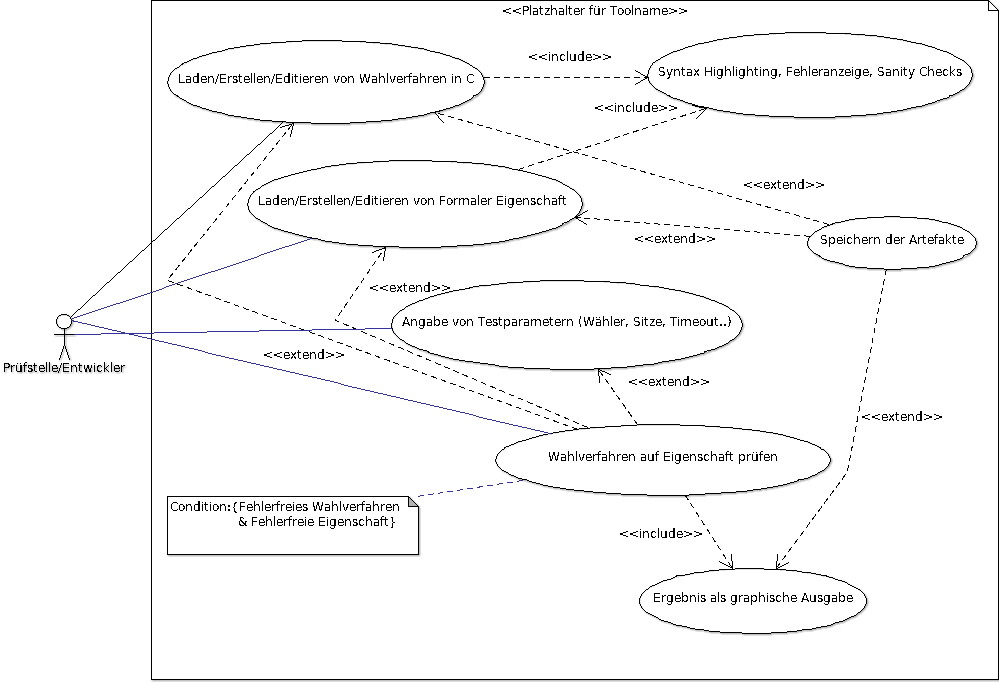
\includegraphics[scale=0.49]{Use-Case-Diagram}}
	


\chapter{GUI}
Die hier vorgestellte \ac{GUI} erfüllt alle Muss-, Soll- und Kann-Kriterien. Das endgültige Produkt kann daher davon abweisen. Im Folgenden wird jedes mal darauf hingewiesen, falls es sich bei einem Feature um ein Kann-Kriterium handelt.
Die \ac{GUI} besteht aus 4 verschiedenen Fenstern: 
\begin{itemize}
\item Ein Editor für C-Code, in welchem die Wahlverfahren editiert werden können.
\item Eine Liste, in welcher alle für dieses Wahlverfahren zu überprüfenden Eigenschaften angezeigt werden.
\item Ein Editor in welchem Eigenschaften editiert werden können.
\item Das Hauptfenster, dessen schließen ein Beenden des kompletten tools nach sich zieht. Darin können Parameter für Überprüfungen eingestellt und Überprüfungen gestartet bzw. beendet werden.
\end{itemize}
Jedes dieser Elemente verfügt auch über weitere Eigenschaften, die im Folgenden beschrieben werden.

\section{C-Editor}
Der C-Editor verfügt über dieselbe Funktionalität, welche andere Texteditoren wie zum Beispiel Notepad aufweisen. Ziel ist es das eingeben von Funktionen welche ein Wahlverfahren implementieren zu ermöglichen. Dazu bietet er die Möglichkeit, C-Code zu schreiben und zu bearbeiten. Ein angemessener Funktionskörper, welcher die auswählbare Art der Wahl repräsentiert, wird dabei automatisch generiert (siehe \ref{Editor-mit-text}). Es wird nicht möglich sein, außerhalb dieser Funktion zu editieren. Dies untersagt aufgrund der Natur von C zum Beispiel selbst definierte Funktionen. Während des Eingeben des Codes wird dieser automatisch analysiert, um Schlüsselwörter sowie syntaktische Fehler zu markieren. 
Der C-Editor teilt sich in vier Untereinheiten auf: Der Menüstreifen, die Tool-Leiste, das Textfeld und das Fehlerfeld. Der Menü-Streifen ist unterteilt in Datei, Bearbeiten, Editor (Kann) und Code. Bilder aller Untermenüs geöffnet befinden sich im Anhang. Sie beinhalten folgende Funktionalität:

\begin{table}[H]
\begin{tabular}{lcr} 
Menüpunkt & Bedeutung \\
\hline
Neu & öffnet ein neues Dokument, wobei die Art der Wahl vom User angegeben wird \\
Speichern & speichert das Dokument unter bereits gegebenem Namen \\
Speichern unter & Speichert das Dokument unter neuem Namen an neuem Ort, beide durch User gegeben \\
Öffnen & Öffnet neues Dokument des richtigen Formats
\end{tabular}
\label{Datei-Menüpunkte}
\caption{Unterpunkte des Datei-Menüs}
\end{table}

\begin{table}[H]
\begin{tabular}{lcr} 
Menüpunkt & Bedeutung \\
\hline
Rückgängig & Falls möglich: Macht die letzte ausgeführte Aktion Rückgängig \\
Wiederholen & Wiederholt die zuletzt Rückgängig gemachte Aktion \\
Kopieren & Fügt markierten Text in die Zwischenablage ein \\
Ausschneiden & Fügt markierten Text in die Zwischenablage ein und entfernt ihn aus dem Textfeld \\
Einfügen & Fügt Text aus der Zwischenablage an der Stelle des Cursors ein \\
Wahlart ändern & Ändert den Funktionskörper zu dem der vom User ausgewählten Art
\end{tabular}
\label{Bearbeiten-Menüpunkte}
\caption{Unterpunkte des Bearbeiten-Menüs}
\end{table}

\begin{table}[H]
\begin{tabular}{lcr} 
Menüpunkt & Bedeutung \\
\hline
Einstellungen & Öffnet den Einstellungen Dialog. Dies ist Teil der Kann-Kriterien. Falls implementiert wird es Möglichkeiten zur Einstellung des Fonts und Syntax-Highlighting geben 
\end{tabular}
\label{Editor-Menüpunkte}
\caption{Unterpunkte des Editor-Menüs}
\end{table}

\begin{table}[H]
\begin{tabular}{lcr} 
Menüpunkt & Bedeutung \\
\hline
Statische Analyse & Startet eine statische Analyse des Codes, welche ihn auf von Lexer oder Parser erkennbare Fehler untersucht. Gefundene Fehler werden in dem Fehlerfeld angezeigt. Zusätzliches Kann-Kriterium Die Zeile, in welcher der Fehler ist, wird zusätzlich durch einen roten Punkt markiert (siehe \ref{Editor-mit-Fehler-nach-statischer-analyse}
\end{tabular}
\label{Editor-Menüpunkte}
\caption{Unterpunkte des Code-Menüs}
\end{table}

Über den Tool-Streifen lassen sich einige dieser Aktionen ohne Öffnen eines Menüs ausführen. Von Links nach Rechts: Neu, Rückgängig, Wiederholen, Speichern, Speichern unter, Öffnen, Kopieren, Ausschneiden, Einfügen.

In \ref{Editor-mit-text} sieht man den Editor nach Eingabe diverser Elemente der C-Sprache. Anzeige der Zeilennummern ist Soll-Kriterium, Möglichkeit diese Funktion zu deaktivieren Kann-Kriterium. Die grauen Balken zeigen an dass man nur den Bereich in dem vorgegebenen Funktionskörper editieren kann.

\begin{figure}[H]
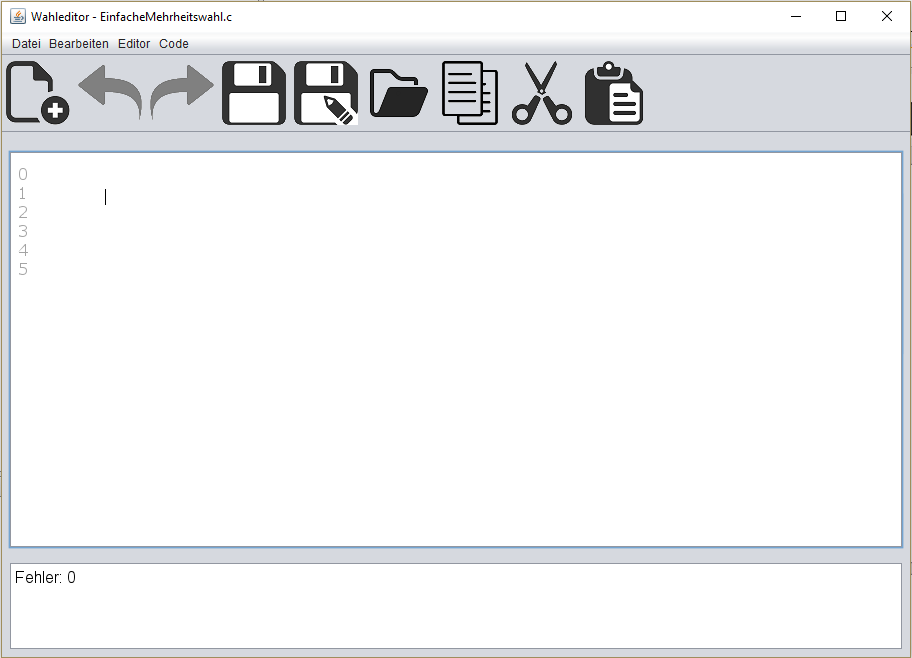
\includegraphics[scale=0.5]{Editor-ohne-text.png}
\caption{Der C Editor ohne Code}
\end{figure}

\begin{figure}[H]
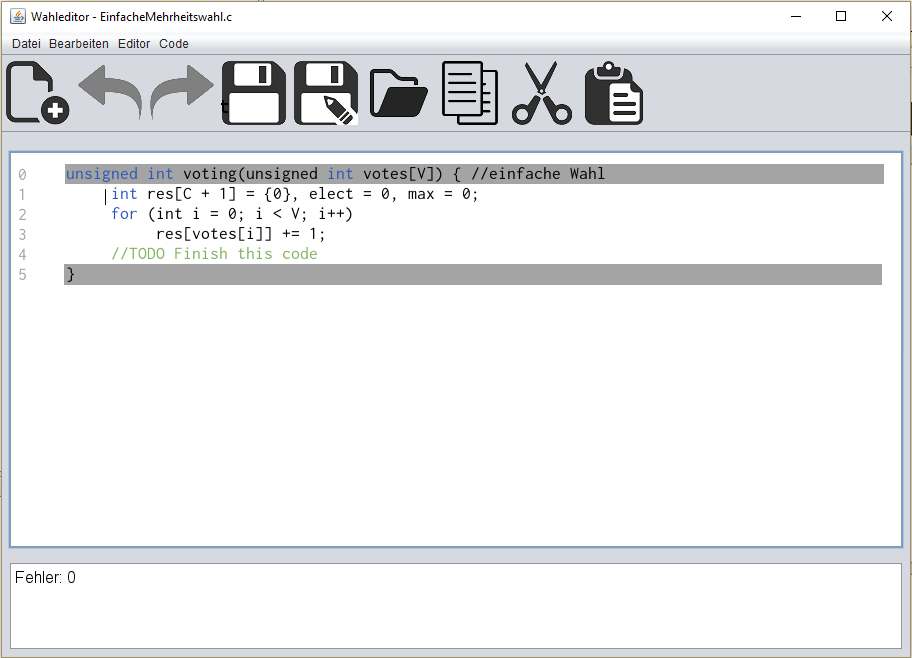
\includegraphics[scale=0.5]{Editor-mit-text.png}
\caption{Der C Editor mit Code und Anzeige der Wahlart}
\label{Editor-mit-text}
\end{figure}

\begin{figure}[H]
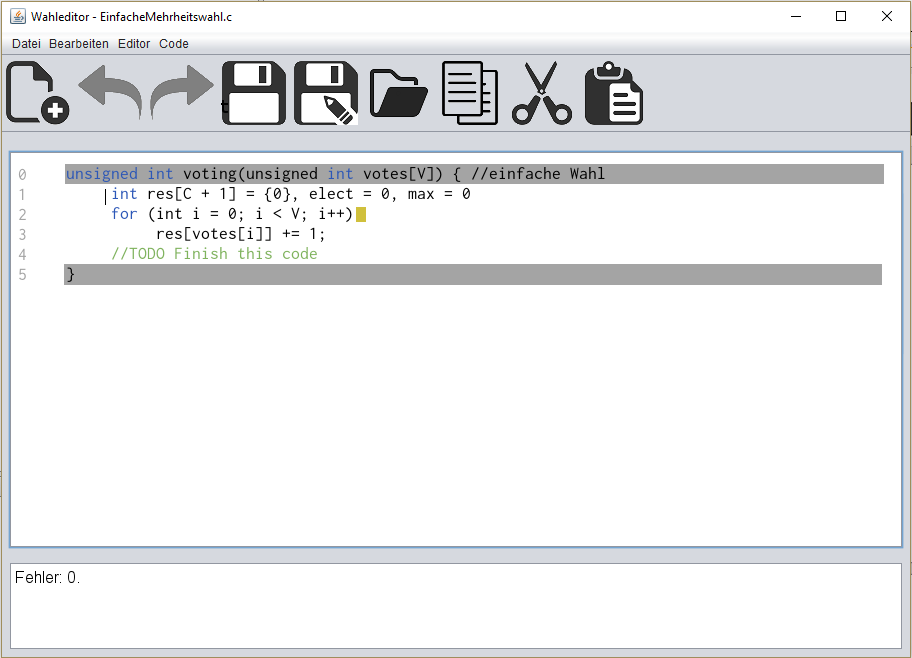
\includegraphics[scale=0.5]{Editor-mit-Fehler-ohne-hover.png}
\caption{Fehleranzeige bei syntaktischem Fehler ohne Maus Hover (Kann-Kriterium)}
\label{Editor-mit-Fehler-ohne-hover}
\end{figure}

\begin{figure}[H]
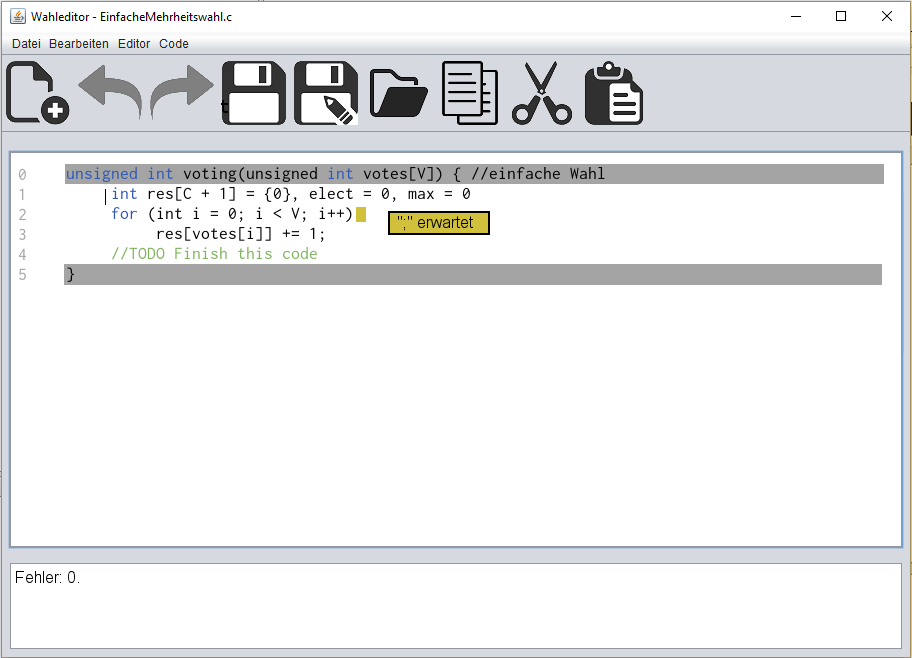
\includegraphics[scale=0.5]{Editor-mit-Fehler-mit-hover.png}
\caption{Fehleranzeige bei syntaktischem Fehler mit Maus Hover (Kann-Kriterium)}
\label{Editor-mit-Fehler-mit-hover}
\end{figure}

In \ref{Editor-mit-Fehler-ohne-hover} sieht man wie der gefundene syntaktische Fehler während des Editieren des Codes angezeigt wird. Dies ist ein Kann-Kriterium. Sobald man mit der Maus über die markierte Stelle geht, wird in einem neuen Fenster nahe der Maus eine Beschreibung des Fehlers angezeigt. Dies ist ebenfalls Kann-Kriterium (siehe \ref{Editor-mit-Fehler-mit-hover}).

\begin{figure}[H]
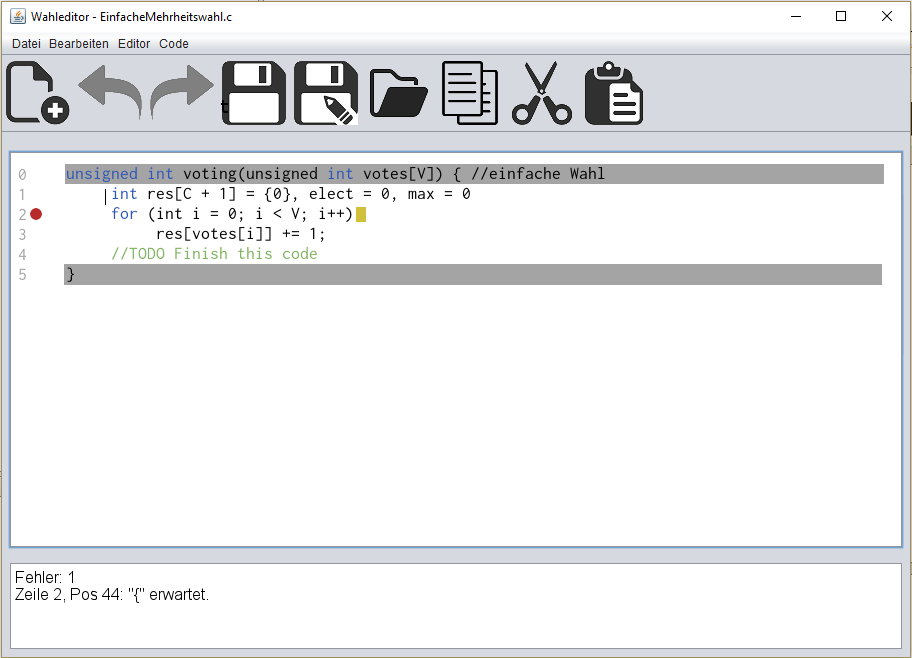
\includegraphics[scale=0.5]{Editor-mit-Fehler-nach-statischer-analyse.png}
\caption{Fehleranzeige nach statischer Analyse}
\label{Editor-mit-Fehler-nach-statischer-analyse}
\end{figure}

\ref{Editor-mit-Fehler-nach-statischer-analyse} Zeigt die Anzeige der Fehler nach ausführend einer statischen Code Analyse. Markierung der Zeile ist Kann-Kriterium.

\section{Eigenschaften-Liste}
Die GUI trennt das Editieren der zu überprüfenden Eigenschaften (in eigens zu diesem Zweck erstellter Syntax, siehe XXX) und das Zuordnen dieser Eigenschaften zu Wahlverfahren. Dadurch können diese Eigenschaften einzeln abgespeichert und flexibel Wiederverwertet und Kombiniert werden. Das Zuordnen zu Wahlverfahren geschieht in der Eigenschaften-Liste. Darin werden die einzelnen Eigenschaften namentlich aufgelistet (siehe ). Im Folgenden werden die einzelnen \ac{GUI}-Bestandteile und der Funktionalität erläutert.

\begin{table}[H]
\begin{tabular}{lcr} 
Menüpunkt & Bedeutung \\
\hline
Neu & Startet eine neue Liste \\
Speichern & Speichert die Liste \\
Speichern unter & Speichert die Liste unter neuem Namen an neuem Ort \\
Öffnen & öffnet Liste (Ort von User angegeben)
\end{tabular}
\label{Eigenschaftenliste-Datei-Menüpunkte}
\caption{Unterpunkte des Datei-Menüs}
\end{table}

\begin{table}[H]
\begin{tabular}{lcr} 
Menüpunkt & Bedeutung \\
\hline
Rückgängig & Falls möglich: Macht die letzte ausgeführte Aktion Rückgängig \\
Wiederholen & Wiederholt die zuletzt Rückgängig gemachte Aktion 
\end{tabular}
\label{Eigenschaftenliste-Bearbeiten-Menüpunkte}
\caption{Unterpunkte des Bearbeiten-Menüs}
\end{table}

Der Tool-Streifen hat exakt den selben Zweck wie der des Code-Editors, ohne die Funktionen Kopieren, Ausschneiden und Einfügen.

\begin{figure}[H]
\begin{minipage}{.5\textwidth}
  \centering
  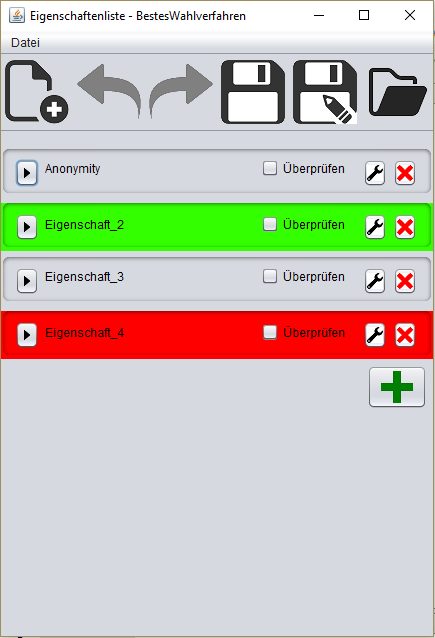
\includegraphics[scale=0.5]{nach-testen.png}
  \captionof{figure}{Liste nach Überprüfung}
  \label{fig:sub1}
\end{minipage}
\begin{minipage}{.5\textwidth}
  \centering
  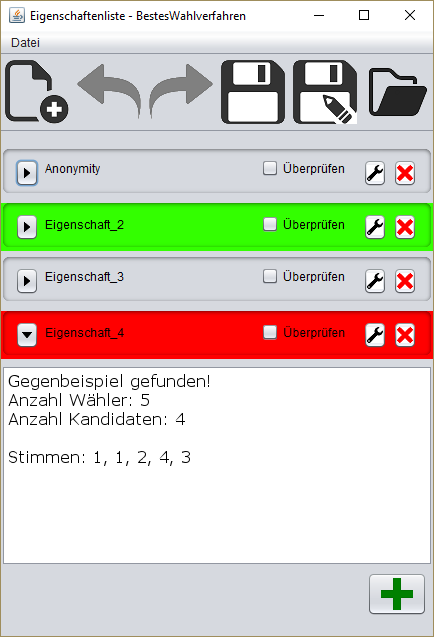
\includegraphics[scale=0.5]{gegenbeispiel.png}
  \captionof{figure}{Anzeige des Gegenbeispiels}
  \label{fig:sub2}
\end{minipage}
\end{figure}

Es folgt eine Beschreibung der Icons, welche zu sehen sind.

\begin{table}[H]
\begin{tabular}{lcr} 
Icon & Bedeutung \\
\hline
Pfeil nach rechts & Falls Gegenbeispiel gefunden: Durch klicken öffnet sich unter dem Listenelement ein Textfeld in welchen das Gegenbeispiel dargestellt wird \\
Checkbox & Nur falls aktiviert, wird das Wahlverfahren auf die Eigenschaft getestet \\
Maulschlüssel & Öffnet den Eigenschaften-Editor für die Eigenschaft\\
Rotes Kreuz & Entfernt die Eigenschaft aus der Liste \\
Gründes Plus & Fügt neue, leere Eigenschaft oder bereits gespeicherte Eigenschaft der Liste hinzu
\end{tabular}
\label{Eigenschaftenliste-Bearbeiten-Menüpunkte}
\caption{Icons der Eigenschaften-Liste}
\end{table}

\section{Eigenschaften Editor}

\begin{figure}[H]
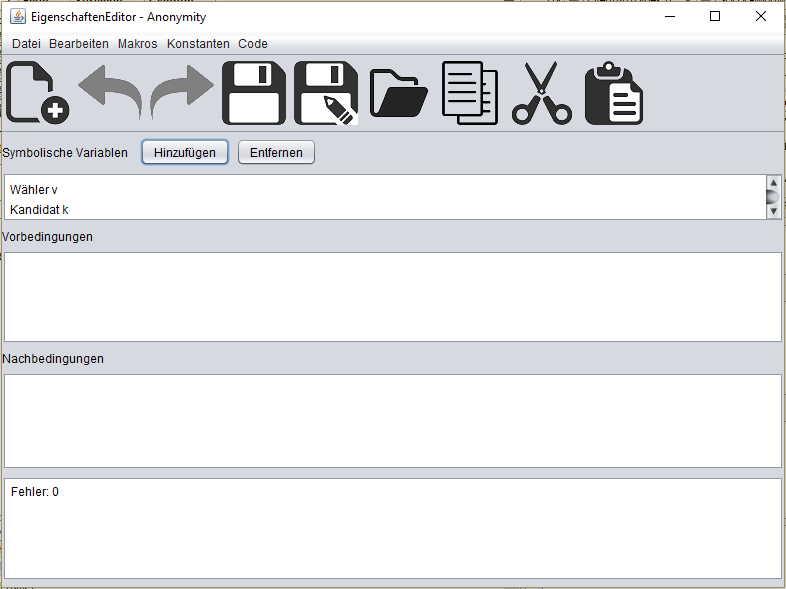
\includegraphics[scale=0.5]{raw-ohne-code.png}
\caption{Eigenschaften-Editor ohne Code mit symbolischen Variablen}
\label{Eigenschaften-Editor-ohne-code}
\end{figure}

Der Eigenschaften-Editor hat den Zweck, das Bearbeiten der zu überprüfenden Eigenschaften zu ermöglichen. Eigenschaften werden aufgeteilt in Vor- und Nachbedingungen. Möglich ist die Verwendung sowohl von Quantoren in der Form von Makros als auch symbolischer Variablen. 

Die Untermenüs Datei, Bearbeiten und Code sowie der Tool-Streifen sind analog zu denen des C-Editors. Hinzu kommen jedoch Konstanten und Makros. Bereitgestellte Konstanten sind: 

\begin{itemize}
\item Die Anzahl der Wähler (V)
\item Die Anzahl der Kandidaten (C)
\item Die Anzahl vorhandener Sitze (S)
\end{itemize}

Bereitgestellte Makros sind:

\begin{itemize}
\item \verb!FOR_ALL_VOTERS()!
\item \verb!FOR_ALL_CANDIDATES()!
\item \verb!FOR_ALL_SEATS()!
\item \verb!EXISTS_ONE_VOTER()!
\item \verb!EXISTS_ONE_CANDIDATES()!
\item \verb!EXISTS_ONE_SEAT()!
\item \verb!SUM_VOTES_FOR_CANDIDATE()!
\end{itemize}

Jedes dieser Makros bis auf das Letzte nimmt eine bisher ungenutzte Variable als Argument. Diese kann im darauf Folgenden boolschen Ausdruck verwendet werden (siehe \ref{Eigenschaften-Editor-Anonymität}). Das Letzte Makro nimmt eine bereits definierte symbolische Variable vom Typ Kandidaten und gibt berechnet die Anzahl Stimmen für diesen Kandidaten.

\begin{figure}[H]
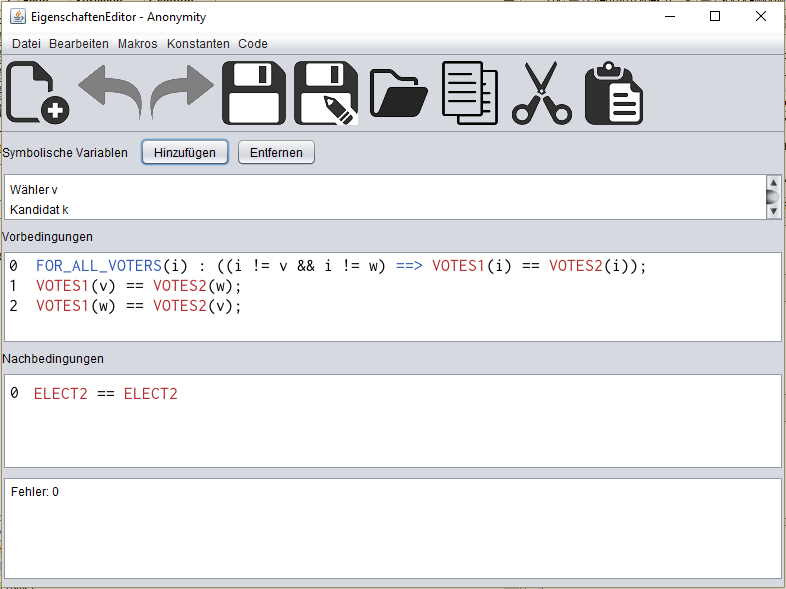
\includegraphics[scale=0.5]{Editor-vor-und-nachbedingungen-syntax-highlighting.png}
\caption{Eigenschaften-Editor mit Beispielhafter Eigenschaft Anonymität und beispielhaft dargestelltem Syntax-Highlighting (Kann-Kriterium)}
\label{Eigenschaften-Editor-Anonymität}
\end{figure}

Wie man zusätzlich sehen kann, sind auch Implikationen (\verb!==>!) möglich. Auch das logische und (\verb!&&!), oder (\verb!||!) und die Äquivalenz (\verb!<==>!) werden zur Verfügung stehen. Die Anzeige erkannter Fehler wird analog zum C-Editor geschehen.

\section{Parameter Editor}

Der Parameter Editor stellt das Hauptfenster der Anwendung dar. Es erlaubt das Einstellen und Starten der Tests. Hier lassen sich auch komplette Projekte Speichern - Code, Eigenschaften und Parameter gebündelt.

\begin{figure}[H]
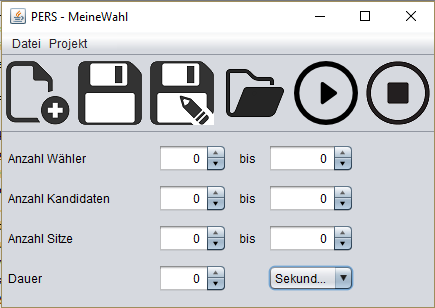
\includegraphics[scale=1]{Parameter-editor.png}
\caption{Der Parameter Editor. PERS steht für Professional Election Rigging System}
\label{Parameter-editor}
\end{figure}

Das Datei Menü ist analog zu dem des C Editors. Das Projekt Menü wird im Folgenden erläutert. 

\begin{table}[H]
\begin{tabular}{lcr} 
Menüpunkt & Bedeutung \\
\hline
Teste Eigenschaften & Startet Tests mit den angegebenen Parametern \\
Stop Test & Unterbricht momentan laufenden Test
\end{tabular}
\label{Parameter-Projekt-Menü}
\caption{Parameter Editor Projekt Menüpunkte}
\end{table}

Der Pfeil und das Stopp-Zeichen des Tool-Streifens haben ebenfalls die Wirkungen Teste Eigenschaften und Stop Test. 

Als Mögliche Zeitangaben stehen Sekunden, Minuten, Stunden und Tage zur Verfügung.

\chapter{Phasenverantwortliche}
\section{Pflichtenheft} Justin Hecht
\section{Entwurf} Holger Klein 
\section{Implementierung} Niels Hanselmann, Nikolai Schnell
\section{Qualitätssicherung} Lukas Stapelbroek
\section{Abschlusspräsentation} Jonas Wohnig

\chapter{Glossar}
 

\printglossaries
 

 
\end{document}